\section{Detection}

Up to here, the \textbf{Segmenter} has finished its work and we have a number of blobs that correspond to the changes in the background. Some of these changes are definitely the objects we are interested in. This step in the tracker mainly focuses on detecting the important parts of these background changes.

The basic detector provided in our framework is based on simple blob detection. It just returns each set of connected pixels as an object. We basically have two questions to investigate about. The first is how the basic tracker provided behave in the presence of noisy detection. The second is how the tracker behaves in the case of no detection. The answers to these two questions are illustrated in the tracking section.

We did several optimizations to the simple detector provided. The first was to detect faces and keep tracking those detected faces. It was used the Viola and Jones AdaBoost Face-Detector[2]. We thought of an interesting application that may use this technique. We added a face recognizer that only detects faces of people of interest to the tracker. We provide a trained Support Vector Machine(SVM) classifier to our tracker. We train it using labeled faces detected from a video for 5 persons. In total 364 faces for 5 people were used for training and all taken from one single video. The \textbf{Detector} then will only detect the people of interest in any video and the tracker will only track those people.

\begin{figure}[Face detection and recognition]{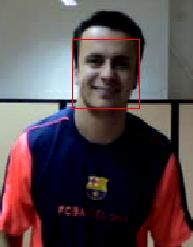
\includegraphics[width=0.3\textwidth]{det_lluis}}
  \centering
  \caption{Face detected and recognized as Lluis}
\end{figure}

In case a match was found, the \textbf{Detector} will return the bounding box of the face that made that match. We thought as an improvement we may try to detect the whole body of the person who made that match. However, plenty of noise coming from the background made this process hard and time consuming. We stopped at this step only satisfied with detecting the face's bounding box and passing it to the \textbf{Representer}.

On the other hand, the \textbf{Detector} may not be able to detect and recognize any face in a certain frame. In this case, the \textbf{Detector} return all those blobs that their \textit{bounding-box} is larger than appropriate threshold. This is done to delete too small noisy blobs and just being interested in those ones that could be a person. The representer will be the responsible to assure if these blobs are belonging to people who was tracked in the last frame.